%
% 03_auswertung.tex -- Beispiel-File für teil2 
%
% (c) 2020 Prof Dr Andreas Müller, Hochschule Rapperswil
%
% !TEX root = ../../buch.tex
% !TEX encoding = UTF-8
%
\section{Visuelle Darstellung der Flussüberquerung
\label{schwimmen:section:bildliche_darstellung}}
\kopfrechts{Visuelle Darstellung der Flussüberquerung}
\begin{figure}
    \centering
    \begin{subfigure}{0.48\textwidth}
        \centering
        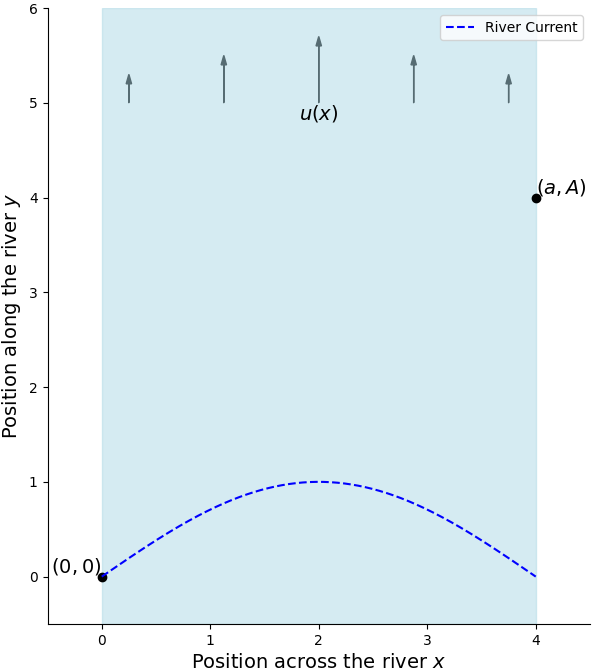
\includegraphics[width=\textwidth]{papers/schwimmen/Grafiken/Figure_2-crop.png}	
        \caption{Flussströmung}
        \label{fig:no_velocity}
    \end{subfigure}
    \hfill  
    \begin{subfigure}{0.48\textwidth}
        \centering
        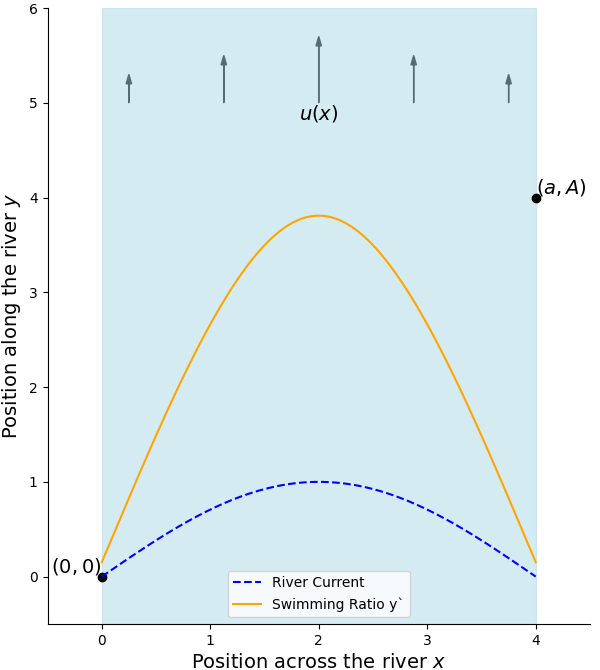
\includegraphics[width=\textwidth]{papers/schwimmen/Grafiken/Figure_3-crop.png}	
        \caption{\(y' = \frac{dy}{dx}\)}
        \label{fig:diagonal_velocity}
    \end{subfigure}
    \par\bigskip
    \begin{subfigure}{0.48\textwidth}
        \centering
        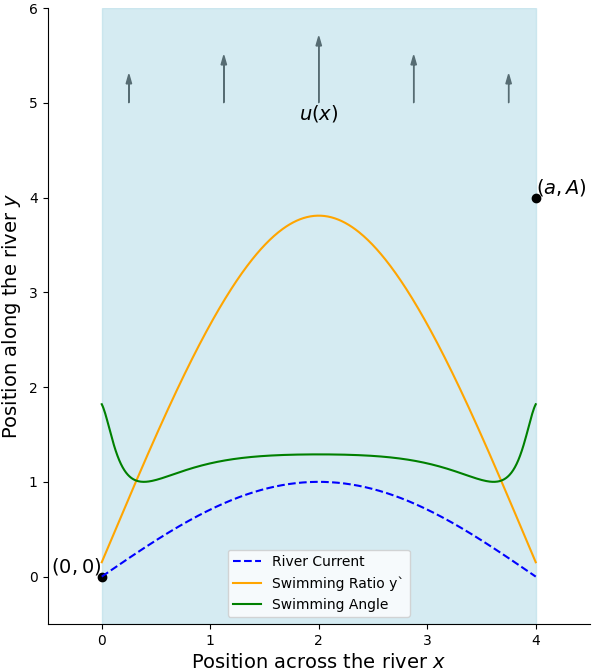
\includegraphics[width=\textwidth]{papers/schwimmen/Grafiken/Figure_4-crop.png}	
        \caption{Winkel der Schwimmenden Person}
        \label{fig:squerd_velocity}
    \end{subfigure}
    \hfill  
    \begin{subfigure}{0.48\textwidth}
        \centering
        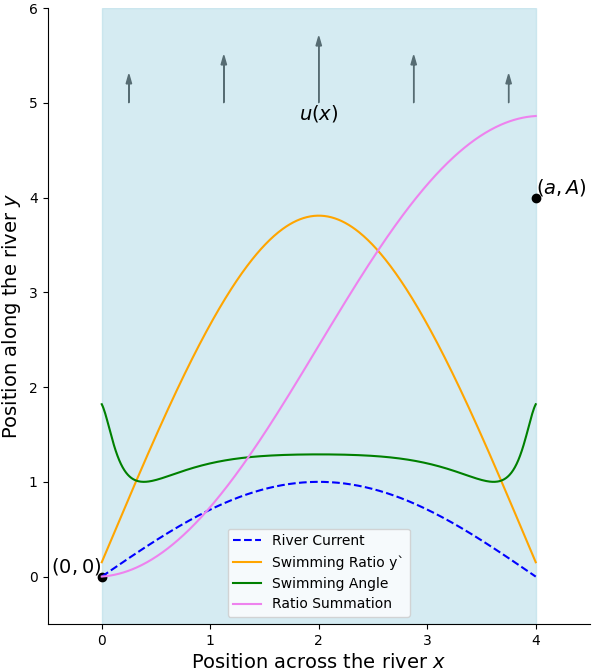
\includegraphics[width=\textwidth]{papers/schwimmen/Grafiken/Figure_5-crop.png}	
        \caption{Aufsumierte Steigung}
        \label{fig:sin_velocity}
    \end{subfigure}
    \par\bigskip
    \caption{Die vier Grafiken stellen verschiedene Graphen dar die für die Flussüerquerung zentrall sind, (a) stellt die Flussströmung dar, (b) das Verhältis zwischen was in \(x\)- und \(y\)-Richtung geschwommen wird, (c) den Winkel der aus dem Verhältnis folgt und (d) das aufsummierte Verhältnis}
    \label{fig:river_pfrofiles}
\end{figure}
%
% papers/schwimmen/


Die Gleichung \eqref{eq:angle} beschreibt das Verhältnis \(\frac{dy}{dx}\)
für die Schwimmrichtung der schwimmenden Person, um die optimale
Flussüberquerung zu erreichen.

In Abbildung \ref{fig:river_pfrofiles} ist eine visuelle Darstellung
für die Flussüberquerung. Es ist zu sehen, dass die Person am
Uferrand weit nach oben schwimmt und dann in der Mitte des Flusses
fast keine Änderung in \(y\)-Richtung macht sondern nur in
\(x\)-Richtung. Sie versucht also, den Bereich stärkerer Strömung,
in der Mitte des Flusses, möglichst schnell hinter sich zu bringen.



